\chapter{Mimicking Non-Monotonic Logics With SCPs} \label{chp:mimick}

\section{The Suppression Task}

\section{The Weak Completion Semantics}



\chapter{Modelling Experiments with SCPs} \label{chp:model}
\section{Overview}
As with any cognitive framework, the most important metric for judging the success of SCPs comes from testing how well SCPs can approximate empirical data across tasks. This chapter will show the suitability of SCPs with a common set of allowable cognitive operations for modelling several well-studied experiments in cognitive modelling.

In particular, we will show that the Wason Selection Task, Suppression Task and @TODO can be modelled at both the general and individual reasoner level with SCPs in a formulation that intuitive and consistent with the WCS approach already described in Section~@TODOref.
\section{Suppression Task}

\begin{figure*}
\begin{center}
 \centering 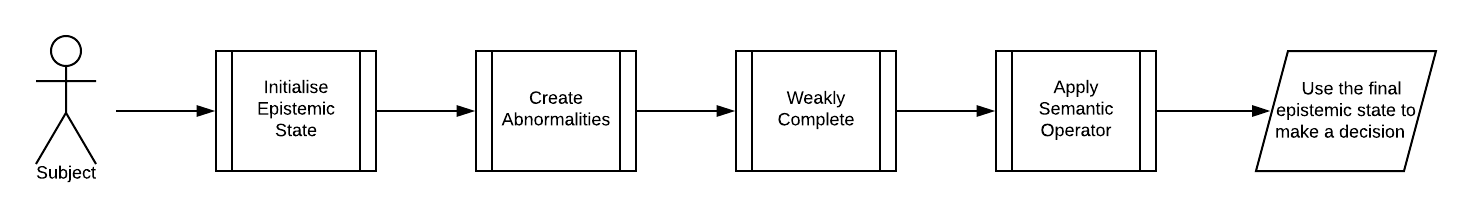
\includegraphics[width=\linewidth]{suppressionSCP_overview}
\caption{A generalised illustration of the WCS in an SCP. }
\label {fig:supoverview}
\end{center}
\end{figure*}

\begin{figure*}
\begin{center}
 \centering 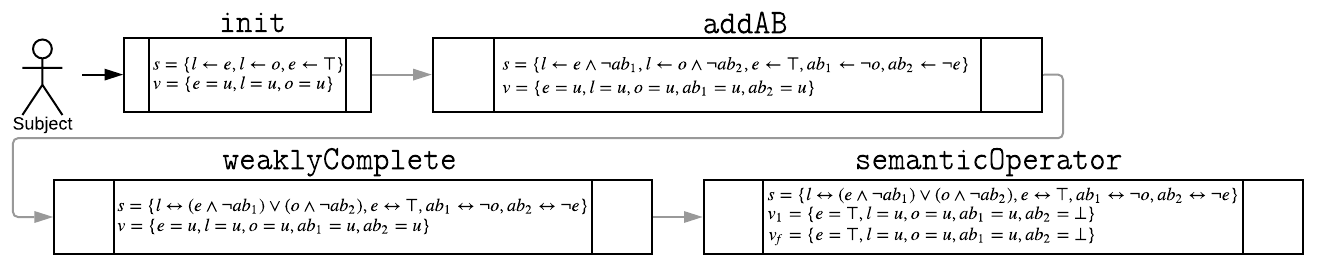
\includegraphics[width=\linewidth]{suppressionSCP_normal}
\caption{The standard case of the Suppression Task, demonstrating the suppression effect. Where the epistemic state in the boxes represents the output of that cognitive operation. $V_f$ represents the assignment of $V$ in the epistemic state in the resulting least model. $V_{i\in \mathbb{N}}$ represents the assignments in $V$ after $i$ iterations of the semantic operator.}
\label {fig:supnormal}
\end{center}
\end{figure*}

Figure~\ref{fig:supoverview} illustrates a generalised SCP to describe the Suppression Task as a series of sequential steps directly mirroring the discrete steps outlined in Section~\ref{sec:sup}, each cognitive operation passing information to the next process\footnote{It is important to note that a diagram like this is valid for \textit{any} cognitive modelling task because any process may be arbitrarily complex and non-sequential. and so the overall linear process of (actor, complex decision, observed results) is always valid for retroactive modelling, and at least as powerful as the non-monotonic logic framework it uses for modelling.}. To model the SCP the implicit sequence of operations in the Suppression Task is systematized and refined into a set of complex operations. Further we introduce an initial epistemic state $s_i=(KB,V,R)$. One interpretation of the requirements of the suppression task $\pi=(s_i,\gamma,M)$ using SCPs and the WCS is as follows: 
 
 
 
 


\[s_i=\{KB_i, V_i, R_i\} \]
\[KB_i=\{e \rightarrow l, \top \rightarrow e, o \rightarrow l\} \]
\[V_i=\{e:u, l:u, o:u\} \]
\[R_i=\{\} \]
\[
\begin{split}
M= \{\texttt{init}, \texttt{addAB}, \texttt{WeaklyComplete}, \texttt{semanticOperator}\}
\end{split}
\]
\[\gamma = (l\models \top) \textrm{ or } (l \models \bot)\]

%@TODO change semanticOper to semanticOperator without line overflowing 

where all cognitive operations require as input and produce as output a state point $p$ where every ground point $\bar{p} \in_s p$ is of format $\bar{p}=(KB,V,R)$; \texttt{init} is always the first cognitive operation and adds the initial variables and rules to epistemic state; \texttt{addAB} adds abnormalities to the current epistemic state using the procedure described in Algorithm~\ref{alg:addAbnormalities} (but now also adds those abnormalities to the variable list of the epistemic state); \texttt{WeaklyComplete} weakly completes the knowledge base of the current epistemic state; and \texttt{semanticOperator} returns an epistemic state that leaves the knowledge base unchanged but updates the variables of that state to return the least model of the epistemic state. \texttt{semanticOperator} follows the same logic seen in Section~\ref{ssec:wcs}, but directly updating $V$ after each iteration of the semantic operator, instead of the externalised variable set $J$. Thus, we ensure that the output state point is able to communicate the result of applying the semantic operator without any structural changes to the epistemic states it contains. As an additional feature of the \texttt{semanticOperator} cognitive operation, if there exists a labelled set in $R$ called $fixed$, then the semantic operator will not set the value of any $v \in fixed$ in the variables list $V$. The goal $\gamma$ states that $l$ should no longer be mapped to unknown in the final epistemic state.



Treating Figure~\ref{fig:supoverview} as an SCP, we observe the sequence of output states seen in Figure~\ref{fig:supnormal}. Note that in the final state $l$ remains mapped to $u$, meaning that the suppression effect is demonstrated.

\subsection{Extending the Suppression Task with SCPs}
The previous example merely showed that SCPs are suitable for modelling the suppression task. In this example we consider one of the most powerful characteristics of SCPs, the ability to model unusual results as deviations from general reasoning. In the original Suppression Task Experiment examined in Section~\ref{sec:sup}, a significant portion of people still believed that she would study late in the library, even though the majority suppressed the inference. Several possible explanations are intuitive, the first and simplest, is the assumption that the reasoner is using classical logic and drawing the classical conclusion. However, what if that is not the case? What if they do reason in exactly the same way as the other reasoners, except for one or two small deviations?

In order to model these non-general reasoners, we consider two possible deviations that could explain the classical result of the Suppression Task: \textit{variable deletion}, and\textit{ variable fixation}. Both of these operations will be discussed in a way that may seem overly prosaic, but it is done to reinforce that we might, reasonably, expect these cognitive operations to occur in day-to-day human cognition.

\subsection*{Variable Deletion} \label{ssec:variableDeletion}
Consider the sequence of numbers: 1, 44, 27, 8, 0 , -4, 6, 7, 346, 7, 74, 7, 234, -55, 2.4, 18. Now without looking back at the numbers, ask yourself some questions: how many numbers were there? Were any of them prime? How many numbers were repeated? In all probability you are not entirely sure. This simple thought experiment provides support for our first extension, the idea that variables can be ``forgotten", that is, that information that existed in the knowledge base at one point in time might no longer exist at a later timepoint. 

This is not the only imaginable case where a variable might be removed from the knowledge base of the person being modelled. The size of the knowledge base used for cognitive modelling is always implicitly restricted to relevant variables. Only those variables whose values might reasonably be expected to affect the final conclusions drawn with regard to the research question should be considered. Finding which variables and rules are relevant is, however, non-trivial. For another real-life example, imagine a mystery novel: Three hundred pages of plot descriptions, character actions, and dialogues. In a good murder mystery novel every piece of information that reveals the killer's identity is hidden in the story itself, yet we do not hold every fact and interaction in the book in our epistemic model of the book, so discerning the identity of the killer remains a mystery until the last page. But when the mystery is solved, many details that we internalised while reading (and recall in retrospect) suddenly make the conclusion seem obvious. We have not forgotten this information, we had merely incorrectly deemed it irrelevant at the time and ignored it in our cognitive processing.

The exact details of how to delete a variable from a knowledge base are non-trivial, and there is no best practice for doing so. But in simple cases the process can be intuitive. Let \texttt{delete} be a complex operation. \texttt{delete} takes as input any state point and is applicable for any ground point $\bar{p}$ with variable list $V \in \bar{p}$ and categorization variable $R$ with ($delete:V_{del}) \in R$, where $V_{del}$ is the set of variable names to delete. For every $v \in V_{del}$ remove all rules from $KB$ that have $v$ as body or head of the clause, and remove $v$ from $V$. Then remove $delete$ from $R$.

In the case of the Suppression Task we argue that one cognitively valid reason for drawing the classical conclusion to the task may be forgetting (or disregarding) the variable $o$. Figure~\ref{fig:supmod} illustrates this case, and shows how the insertion of a complex operation can completely change the final epistemic state.

\begin{figure*}
\begin{center}
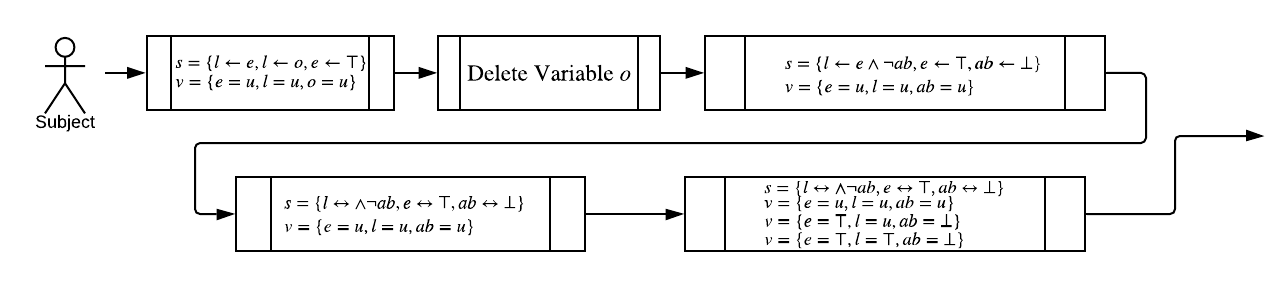
\includegraphics[width=0.85\linewidth]{suppressionSCP_mod}
\end{center}

\caption{The Suppression Task in which the additional operation of deleting the variable $o$ occurs.}
\label{fig:supmod}
\end{figure*}

\subsection*{Variable Fixing} \label{ssec:variableFixing}

\begin{figure*}
\begin{center}
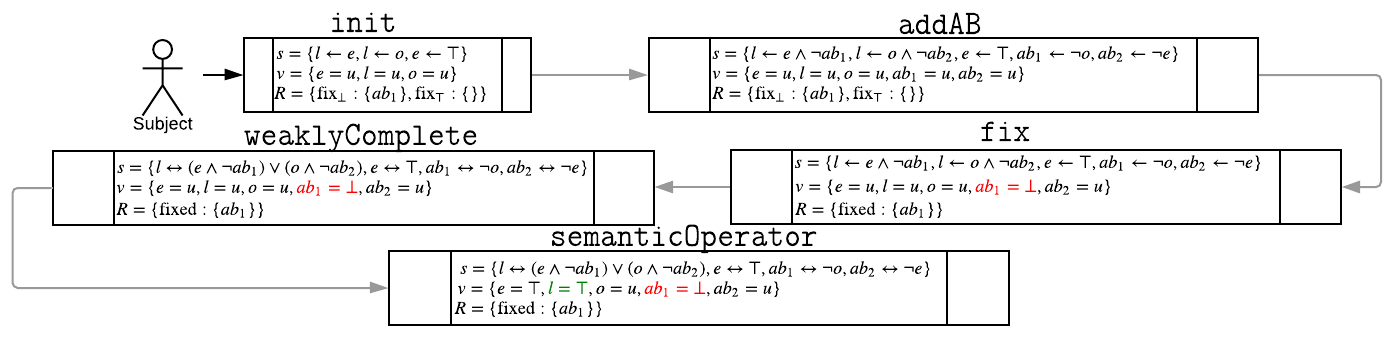
\includegraphics[width=\linewidth]{suppressionSCP_mod2}
\end{center}

\caption{The Suppression Task in which the additional operation of fixing the variable $ab_1$ to false occurs.}
\label{fig:supmod2}
\end{figure*}

The second case of a potential complex operation to add to the search space of our SCPs is the idea of Variable Fixing. The idea that some  conclusions can be fixed \textit{a priori}. Consider a person who strongly doubts the effectiveness of vaccines, we will call her Karen. Karen started her day convinced that giving her child the MMR vaccine is more dangerous than the disease itself. Later that day Karen spoke to her doctor who strongly advised that she vaccinate her child. He offered her a variety of peer-reviewed papers and studies that showed the relative safety of the vaccination. Karen listened carefully to the trained medical professional, and then went home. After some thought Karen decided that he was wrong, and her opinion on vaccines didn't change.

In this example Karen shows a very powerful type of cognitive bias, the unwillingness to change her opinions, despite powerful evidence to the contrary. This phenomenon has been observed across a great many fields of study, from medical psychology \citep{brown2010omission} \citep{wroe2005feeling} to political sciences\citep{tappin2017heart}. In the context of cognitive modelling with logics, it indicates that some mental rules or variables are immutable, regardless of new evidence or valid beliefs that would logically contradict them. Non-monotonic logics, as a class, are already capable of dealing with bias effects, as non-monotonic logics are built on the basis of a preference operation.

 As one possible implementation of this idea, let us introduce a cognitive operation called \texttt{fix}. Fix takes as input any state point and is applicable for any ground point $\bar{p}$ with variable list $V \in \bar{p}$ and categorization variable $R$ with ($fix_\top \lor fix_\bot) \in R$. For all variables $v$ such that $(v \in V) \cap (v \in fix_\top)$ set the value of $v$ to $\top$, For all variables $v$ $(v \in V) \cap (v \in fix_\bot)$ set the value of $v$ to $\bot$. Then remove $fix_\top$ and $fix_\bot$ from $R$. Append $fixed:V_{fix}$ to $R$, where $V_{fix}$ is the set of all variables fixed in this way.

Now, because \texttt{semanticOperator} does not change the values of variables mentioned in $V_{fix} \in fixed:V_{fix}$, $fixed \in R$, Figure~\ref{fig:supmod2} shows the effect of adding a complex operation which fixes the value of the abnormality to false in $v$ so that, no matter what rules in $KB$ when the semantic operator is applied, $ab_1$ will remain false.
\section{Wason Selection Task}